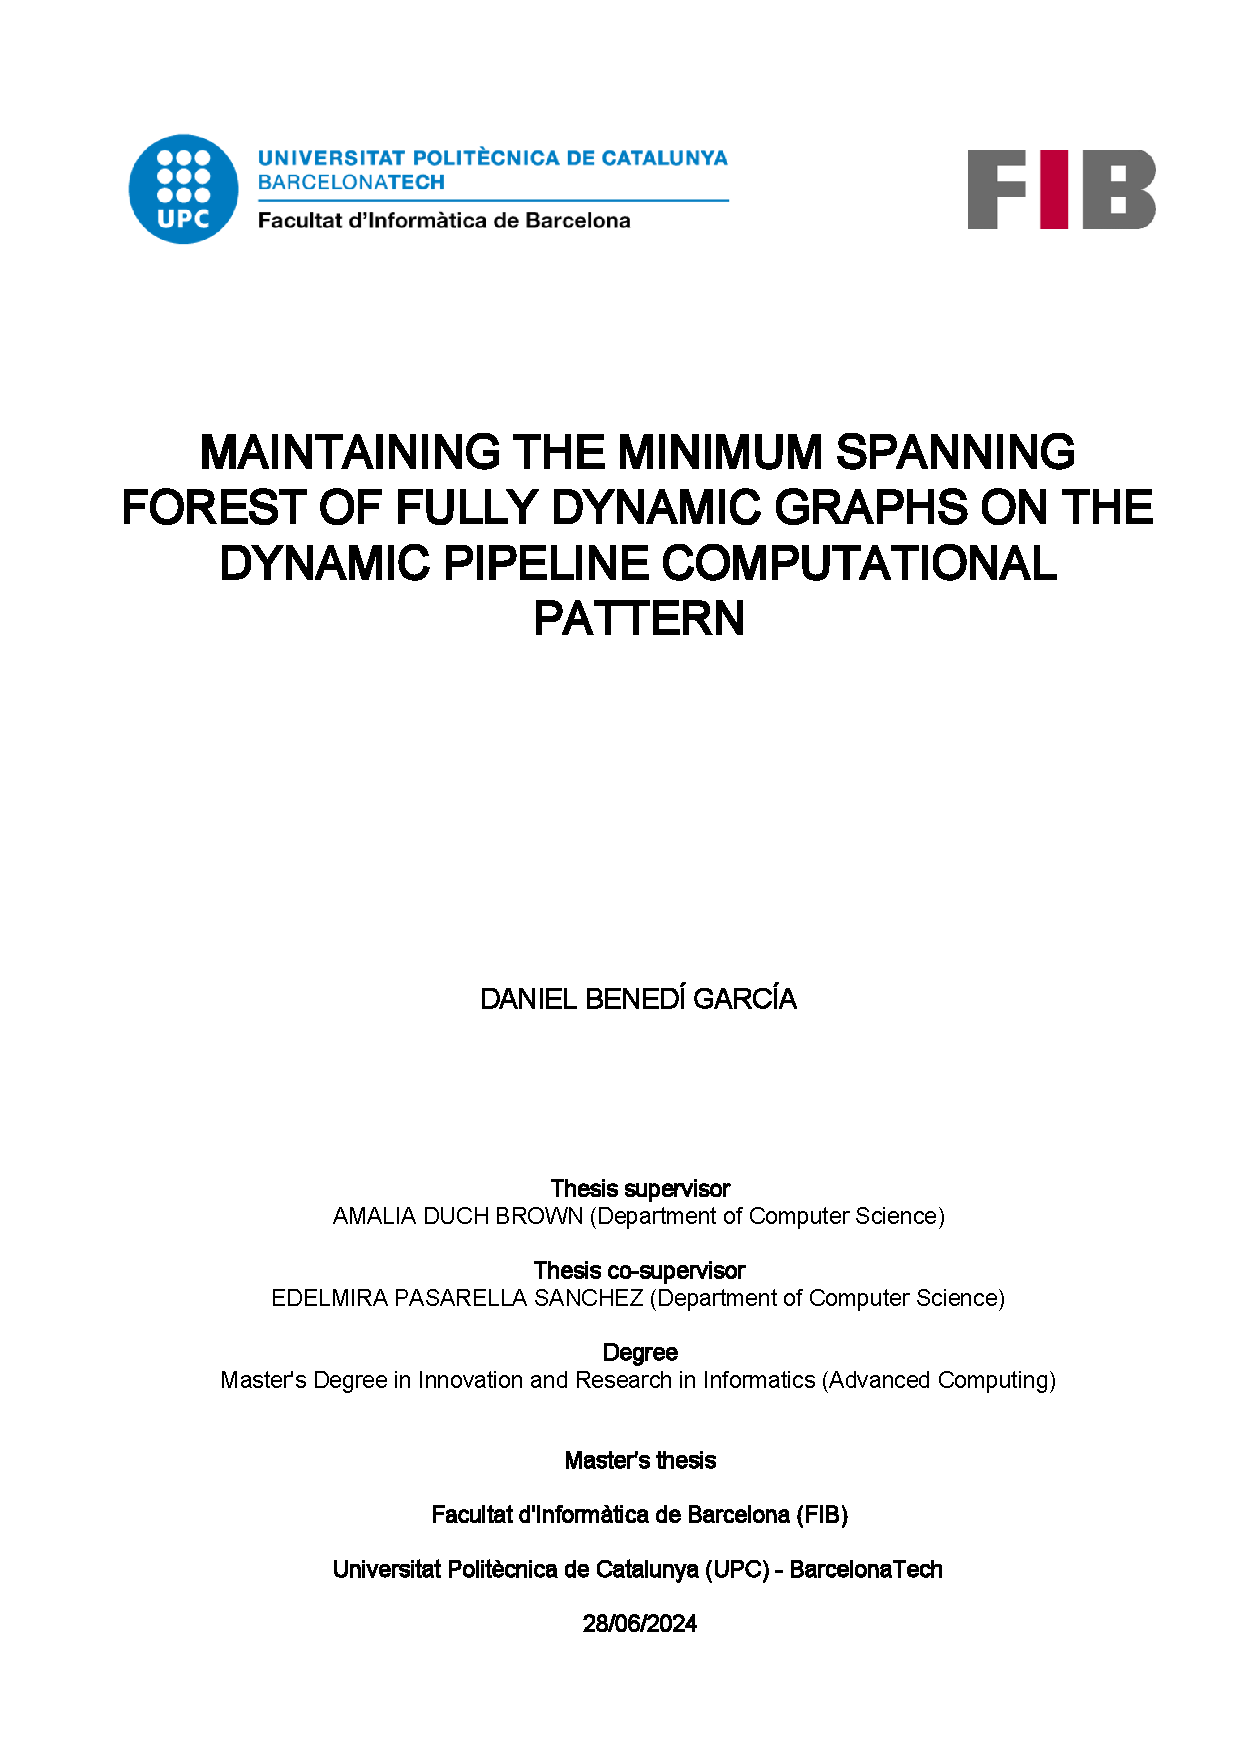
\includepdf{cover.pdf}

\newpage
\thispagestyle{plain}
\begin{flushright}
    
\includegraphics[width=0.8\textwidth]{figures/science.jpg}\\
    I have attempted science - Strange Planet. Nathan W Pyle
\end{flushright}

\newpage

%%%%%%%%%%%%%%%%%%%%%%%%%%%%%%%%%%%%
%%  The English abstract          %%
%%%%%%%%%%%%%%%%%%%%%%%%%%%%%%%%%%%%
\chapter*{Abstract}
%%%%%%%%%%%%%%%%%%%%%%%%%%%%%%%%%%%%
%This work studies the application of the Dynamic Pipeline Approach to parallelize Kruskal's algorithm and thus compute and maintain the Minimum Spanning Tree of dynamic graphs in parallel and distributed settings. To achieve this, we propose to represent the graph through its underlying forest; an adequate representation that enables to store the graph distributed in a dynamic pipeline.
In this work we tackle the problem of using the Dynamic Pipeline Approach to parallelize the Kruskal’s algorithm and thus compute and maintain the Minimum Spanning Tree of dynamic graphs in parallel and distributed settings. To achieve this, we introduce a characterization of  graphs that we call an \emph{underlying forest} of a graph. This characterization gives the basis for representing graphs  in a distributed way along a dynamic pipeline. 

The proposed algorithm, named \DPmst, utilizes a pipeline architecture where the graph is partitioned into trees and distributed across a sequence of stages each handling different aspects of computation. Under this algorithm it possible to keep efficiently graph updates as well as to apply Kruskal's Algorithm at every stage of the pipeline to compute incrementally the minimum spanning tree of the stored graph.

A working implementation was developed to analyze the suitability of \DPmst\ against other algorithms. The programming language \Go\ was chosen because of its concurrency features, as its {\tt goroutines} and  communication channels naturally align with the Dynamic Pipeline Approach.

Several key optimizations were introduced in \DPmst. Some of them regarding the implementation and others the Dynamic Pipeline Approach. Notably, we propose a way to disentangle the message passing from computational tasks which is a general optimization that enhances the entire Dynamic Pipeline Approach framework, not just for \DPmst. These optimizations not only improve program's efficiency but also address and resolve memory management issues within \Go.

Extensive experimental evaluations were conducted to compare \DPmst\ with both sequential and parallel algorithms. Kruskal's algorithm was selected for sequential comparisons, while \FKruskal\ and a message-passing implementation of {\tt Prim}'s algorithm for parallel algorithms. The results demonstrate that \DPmst\ significantly outperforms its counterparts in both single-core and parallel environments, showcasing its superior performance and scalability for handling large and dynamic graphs. 

This work substantiates the effectiveness of the Dynamic Pipeline Approach in addressing complex graph problems and underscores its potential for wider application in parallel computing.


\chapter*{Acknowledgements}
%%%%%%%%%%%%%%%%%%%%%%%%%%%%%%%%%%%%
I would like to express my deepest appreciation to the supervisors of this work, Amalia Duch and Edelmira Pasarella, for their invaluable patience, insightful feedback, and refreshing motivation throughout this journey. Your guidance has been instrumental in the completion of this project.

Additionally, I extend my sincere thanks to the /RDLab-UPC for providing the computational resources necessary for the experimental evaluation. Your support made the technical aspects of this research possible.

I am also grateful to my colleagues and friends from the master program. You provided a warm welcome to this new step in my life, tolerated my moments of stress, and inspired me to dream big. And to my friends from Zaragoza for accompanying me up to this point no matter what happened.

Last but not least, I could not have undertaken this journey without my family and their constant support throughout this research. To my parents, thank you for always supporting me and allowing me to return to my roots; to my sister, for being a beacon of inspiration; and to my significant other, for your constant love and understanding.




\tableofcontents
